\documentclass[../manuale-utente.tex]{subfiles}

\begin{document}

\subsection{Requisiti}%
\label{sub:web_app_requisiti}

\begin{description}
    \item[Browser:] Google Chrome 50, Firefox 48, Safari 9.1.
    \item[Necessario:] JavaScript.
\end{description}
\newpage

\subsection{Manuale d'uso}%
\label{sub:manuale-uso-web}

\subsubsection{Pagina home}%
\label{subs:pagina_home}

\begin{figure}[H]
    \centering
    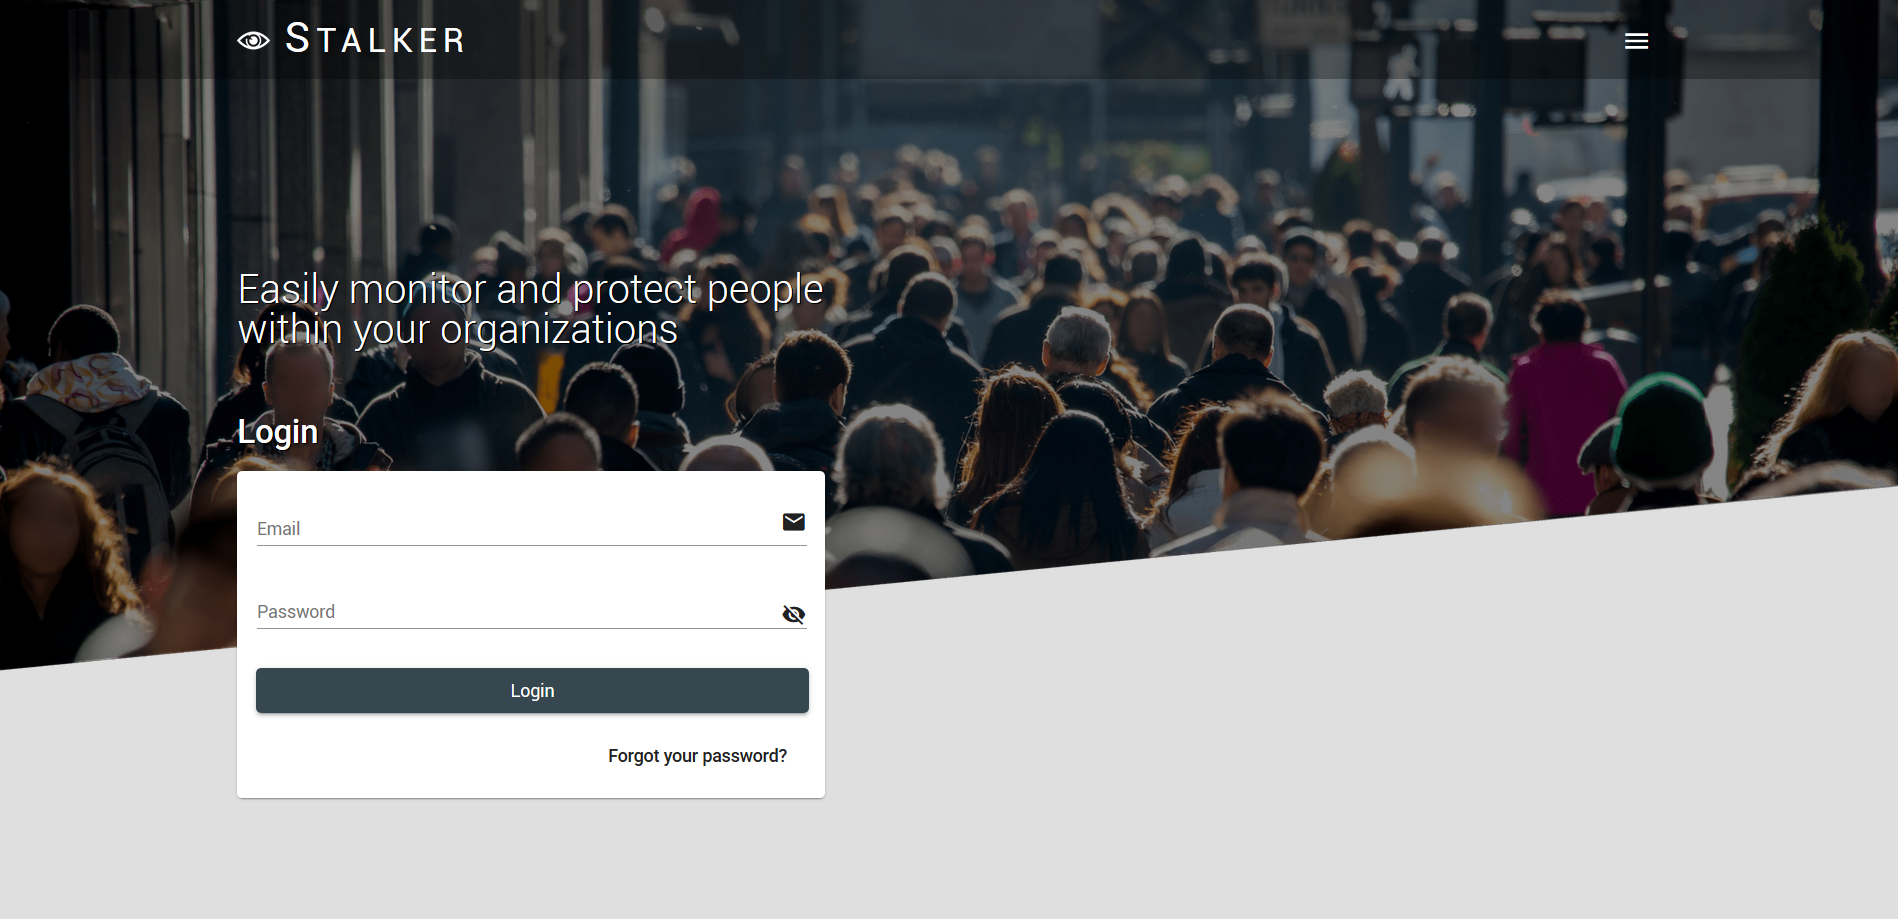
\includegraphics[width=175mm]{pagina-home.png}
    \caption{Pagina di accesso}%
    \label{fig:web_app_pagina_accesso}
\end{figure}

Quando ci si connette alla web application di Stalker, l'utente viene indirizzato alla pagina principale (Home) che si trova al link \textit{localhost:4200/home}.

L'utente non è autenticato e ha le seguenti modalità d'azione:
\begin{itemize}
    \item essere registrato alla web app di Stalker e accedere con le proprie credenziali email e password (~\ref{fig:web_app_form_accesso}).
    \item recuperare la password nel caso l'abbia smarrita (~\ref{fig:web_app_form_recupero_password}).
    \item selezionare il menu ad hamburger posizionato sulla barra superiore a destra, per visualizzare le informazioni riguardo a Stalker. Questo menu è sempre presente in ogni pagina.
\end{itemize}
\newpage

\paragraph{Accesso alla web application}%
\label{par:accesso_alla_web_application}

\begin{figure}[H]
    \centering
    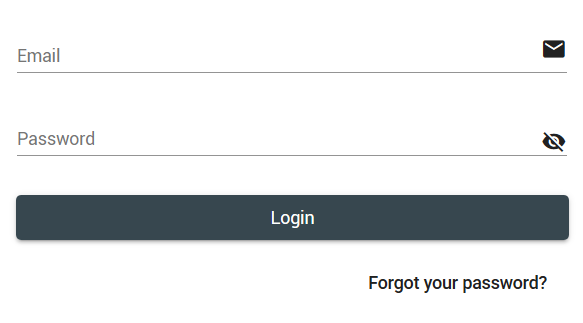
\includegraphics[width=120mm]{accesso-web-app.png}
    \caption{Form di accesso alla web application di Stalker}%
    \label{fig:web_app_form_accesso}
\end{figure}

L'utente vuole accedere al sistema di Stalker, quindi deve eseguire i seguenti passaggi:
\begin{itemize}
    \item inserire correttamente l'email.
    \item inserire la password che deve contenere almeno 8 caratteri (almeno una lettera maiuscola, una lettera minuscola, un numero ed un simbolo) e al massimo ne può contenere 32. La password può essere visualizzata normalmente durante la sua digitazione, cliccando sull'occhio barrato alla fine del campo d'inserimento.
    \item selezionare il pulsante \textbf{Login} per inviare le credenziali al server.
\end{itemize}

% E' corretto?
Nel caso l'operazione venga svolta correttamente, si avrà diritto all'accesso nella web application di Stalker, visualizzando la pagina del profilo personale (~\ref{fig:web_app_visualizza_profilo_personale}).

In caso contrario, l'utente non è autorizzato, in quanto la procedura è fallita.

Le cause possono essere le seguenti:
\begin{itemize}
    \item l'email inserita non rispetta i vincoli imposti dal sistema di Stalker.
    \item la password non rispetta i vincoli imposti dal sistema di Stalker.
    \item l'email e la password inserite non rispettano i vincoli imposti dal sistema di Stalker.
    \item l'email e la password inserite rispettano i vincoli, ma non sono presenti all'interno del database di Stalker.
\end{itemize}

In ogni caso, il messaggio di errore non sarà specifico ma generico, per motivi di sicurezza.
\newpage

\paragraph{Recupero password}%
\label{par:recupero_password}

\begin{figure}[H]
    \centering
    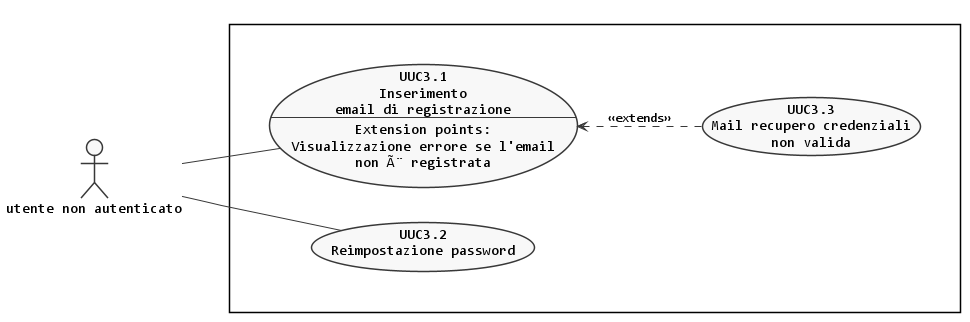
\includegraphics[width=150mm]{recupero-password.png}
    \caption{Form recupero password}%
    \label{fig:web_app_form_recupero_password}
\end{figure}

L'utente ha smarrito la password o non se la ricorda più, quindi deve eseguire tre passaggi:
\begin{itemize}
    \item cliccare alla voce \textbf{Forgot your password?} presente nel form per l'accesso alla web application (~\ref{fig:web_app_pagina_accesso}).
    \item inserire correttamente l'email.
    \item selezionare il pulsante \textbf{Recover} per inviare la richiesta al server.
\end{itemize}

Nel caso l'operazione venga svolta correttamente, l'utente riceverà una mail sulla propria casella postale contenente il link per il recupero della password.

In caso contrario, l'utente non può recuperare la password, in quanto la procedura è fallita.

Le cause possono essere le seguenti:
\begin{itemize}
    \item l'email inserita non rispetta i vincoli imposti dal sistema di Stalker.
    \item l'email inserita rispetta i vincoli, ma non è presente nel database di Stalker, quindi non si può avviare la procedura.
\end{itemize}

In ogni caso, il messaggio di errore non sarà specifico ma generico, per motivi di sicurezza.
\newpage

\subsubsection{Visualizza profilo personale}%
\label{subs:visualizza_profilo_personale}

\begin{figure}[H]
    \centering
    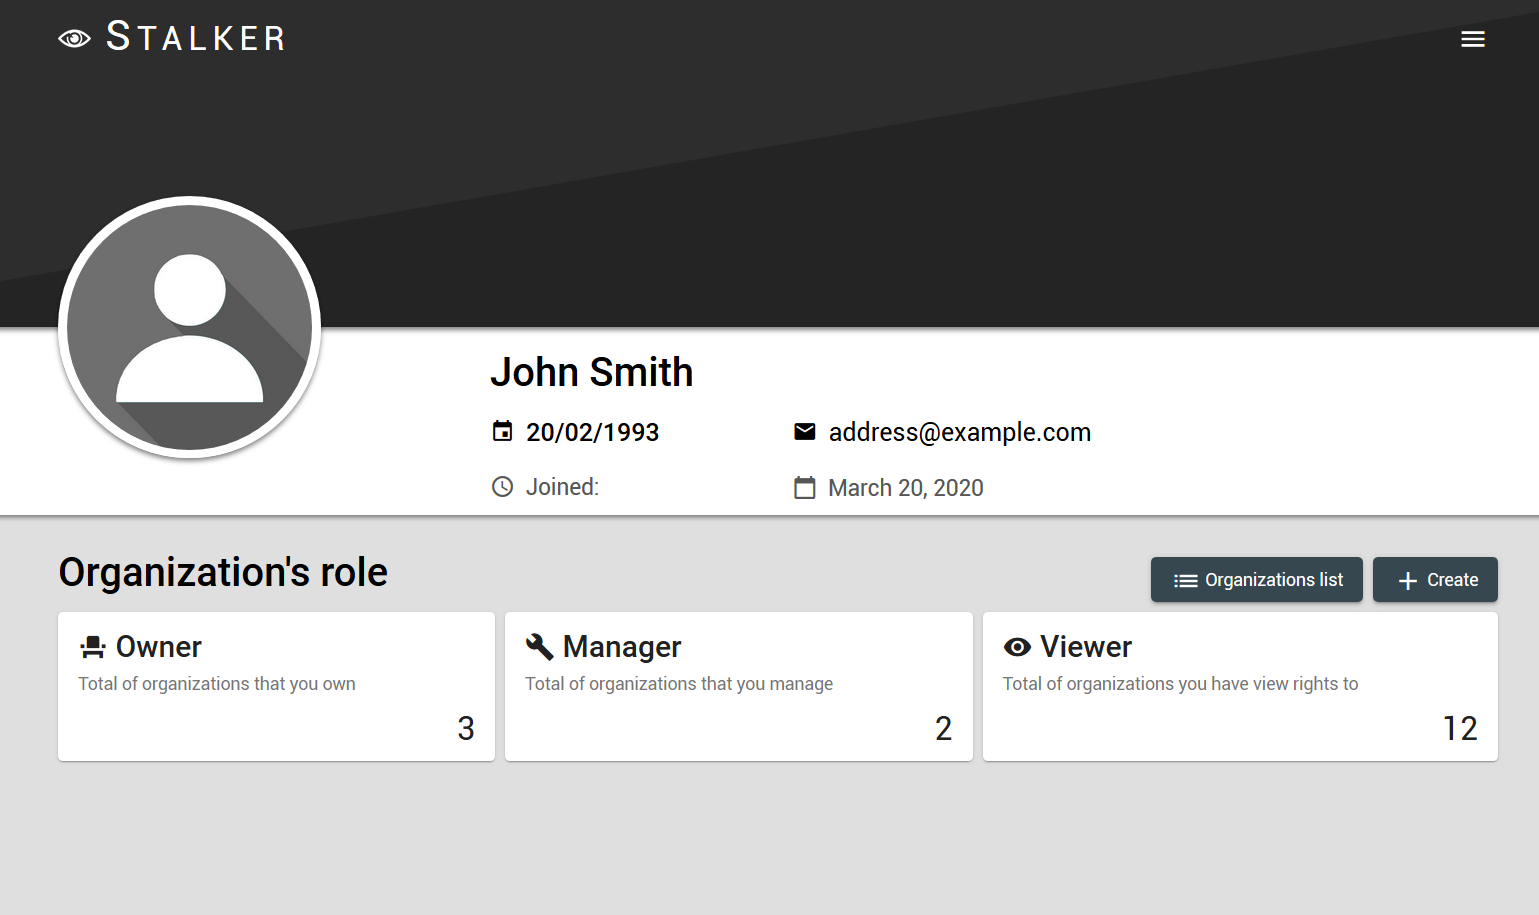
\includegraphics[width=120mm]{visualizza-profilo-personale.png}
    \caption{Visualizza profilo personale}%
    \label{fig:web_app_visualizza_profilo_personale}
\end{figure}

L'utente ha appena effettuato l'autenticazione alla web application di Stalker, quindi si ritrova nella pagina del profilo personale.

I dati che la pagina mette a disposizione dell'utente sono:
\begin{itemize}
    \item una foto profilo.
    \item nome e cognome.
    \item la data di nascita.
    \item l'email con la quale è registrato in Stalker.
    \item il giorno in cui l'utente è stato aggiunto in Stalker.
    \item un'insieme di dati relativi ai ruoli che l'utente possiede in alcune delle organizzazioni di Stalker.
    \begin{itemize}
        \item il numero totale di organizzazioni in cui è owner.
        \item il numero totale di organizzazioni in cui è manager.
        \item il numero totale di organizzazioni in cui è viewer.
    \end{itemize}
\end{itemize}

Inoltre, la seguente pagina fornisce alcune operazioni:
\begin{itemize}
    \item la visualizzazione della lista di tutte le organizzazioni, cliccando il pulsante \textbf{Organizations list}. %(~\ref{fig:web_app_visualizza_organizzazioni}).
    \item la creazione di una nuova organizzazione, cliccando il pulsante \textbf{Create}. %(~\ref{fig:web_app_creazione_organizzazione}).
\end{itemize}
\newpage

\subsubsection{Visualizza organizzazioni}%
\label{subs:visualizza_organizzazioni}

% \begin{figure}[H]
%     \centering
%     \includegraphics[width=120mm]{visualizza-organizzazioni.png}
%     \caption{Visualizza organizzazioni}%
%     \label{fig:web_app_visualizza_organizzazioni}
% \end{figure}

% \textbf{Endpoint}: localhost:4200/organizations
Lorem ipsum
\newpage

\paragraph{Visualizza dettagli organizzazione}%
\label{par:visualizza_dettagli_organizzazione}

\begin{figure}[H]
    \centering
    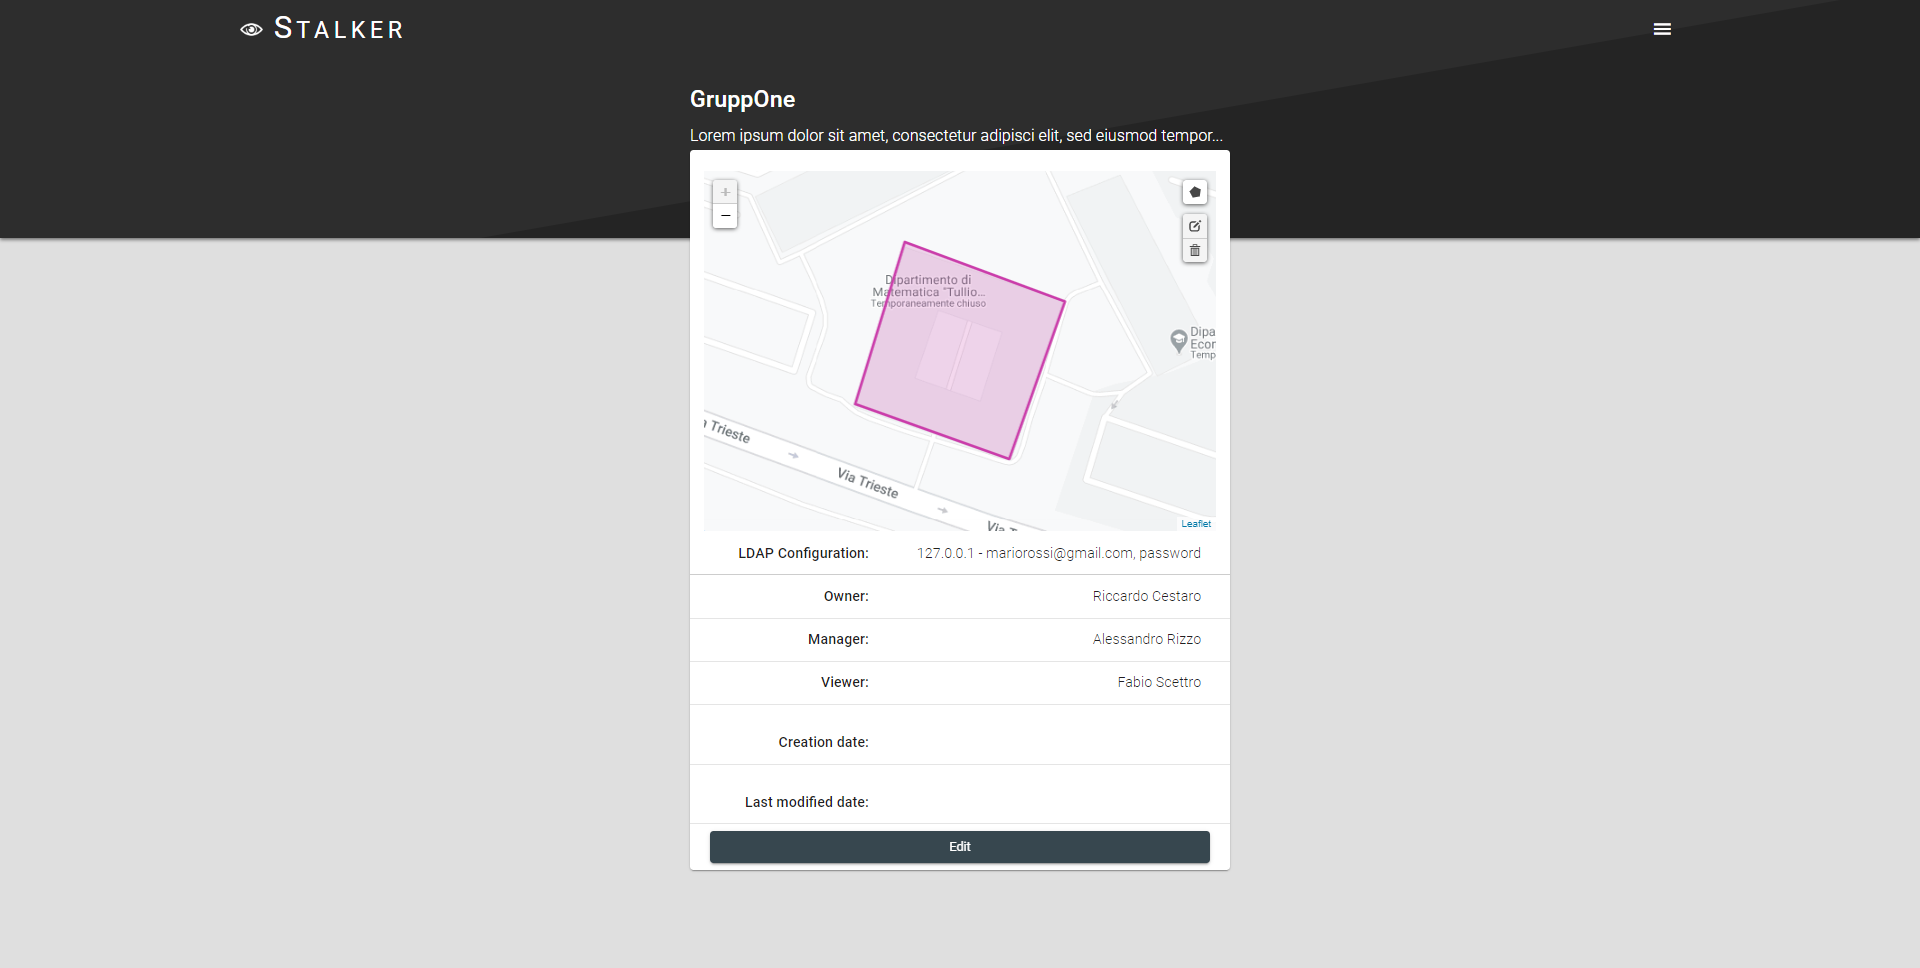
\includegraphics[width=120mm]{visualizza-dettagli-organizzazione.png}
    \caption{Visualizza dettagli organizzazione}%
    \label{fig:web_app_visualizza_dettagli_organizzazione}
\end{figure}

Una volta che l'utente seleziona un'organizzazione dalla lista di organizzazioni, viene indirizzato in un'altra pagina che riporta i dettagli dell'organizzazione selezionata.

I dati che la pagina mette a disposizione sono, dall'alto verso il basso:
\begin{itemize}
    \item il nome dell'organizzazione.
    \item una descrizione relativa all'organizzazione.
    \item una mappa dei luoghi che appartengono all'organizzazione, evidenziati con colori diversi per mostrarli chiaramente sulla mappa.
    \item la configurazione del \glossarioLocale{server LDAP}, presente solo se l'organizzazione è privata e quindi richiede un'autenticazione per l'accesso ad essa.
    \item nome e cognome degli utenti che sono owner dell'organizzazione.
    \item nome e cognome degli utenti che sono manager dell'organizzazione.
    \item nome e cognome degli utenti che sono viewer dell'organizzazione.
    \item la data di creazione dell'organizzazione.
    \item la data dell'ultima modifica applicata alle informazioni dell'organizzazione.
\end{itemize}

Inoltre, viene fornita la possibilità di modificare le informazioni dell'organizzazione cliccando il pulsante \textbf{Edit}, venendo così indirizzati alla pagina di modifica (~\ref{subs:modififica_dettagli_organizzazione}).

Bisogna evidenziare che la modifica di questi dati è consentita solo agli utenti che ne hanno il diritto.
\newpage


\subsubsection{Creazione organizzazione}%
\label{subs:creazione_organizzazione}

% \begin{figure}[H]
%     \centering
%     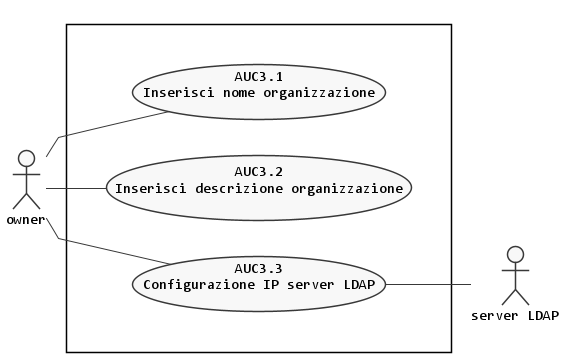
\includegraphics[width=120mm]{creazione-organizzazione.png}
%     \caption{Creazione organizzazione}%
%     \label{fig:web_app_creazione_organizzazione}
% \end{figure}

% \textbf{Endpoint}: localhost:4200/organizations
Lorem ipsum
\newpage

\subsubsection{Modifica dettagli organizzazione}%
\label{subs:modififica_dettagli_organizzazione}

L'utente necessita la modifica dei dettagli di un'organizzazione, che può avvenire in 5 passaggi sequenziali.

Ogni passaggio è identificato da un numero progressivo che va da 1 a 5, inserito all'interno di un cerchio, che è colorato di blu per i passaggi precedenti effettuati e quello corrente, mentre è colorato di grigio per i passaggi successivi che devono ancora essere effettuati.

I 5 passaggi per la modifica sono i seguenti:

\begin{enumerate}
    \item \textbf{Organization details}

    \begin{figure}[H]
        \centering
        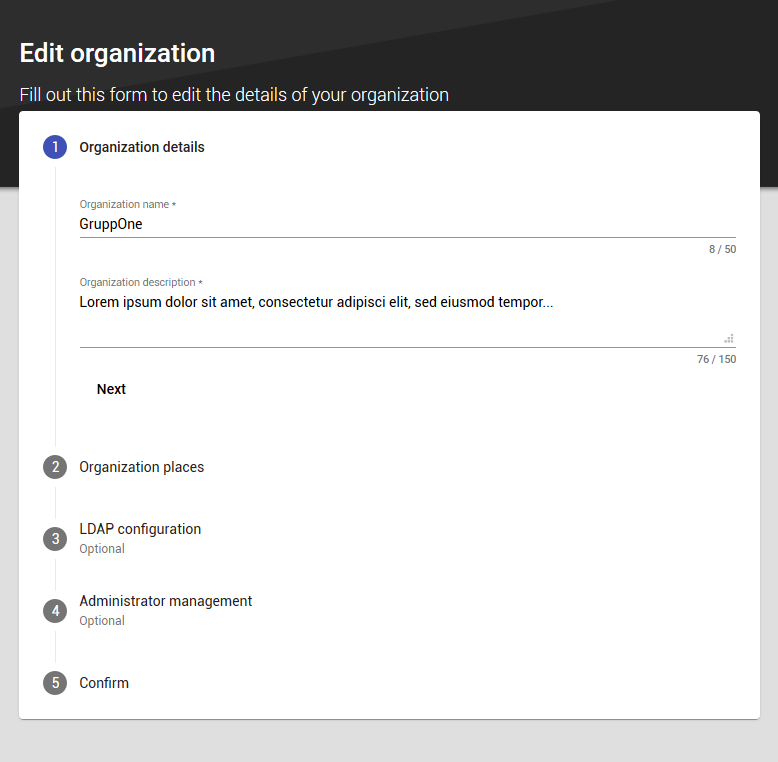
\includegraphics[width=120mm]{1-dettagli-organizzazione.png}
        \caption{Modifica dettagli dell'organizzazione}%
        \label{fig:web_app_modifica_dettagli_organizzazione}
    \end{figure}

    I campi che possono essere modificati sono:
    \begin{description}
        \item[Organization name] che corrisponde al nome dell'organizzazione.
        \item[Organization description] che corrisponde alla descrizione dell'organizzazione.
    \end{description}

    Cliccando \textbf{Next} si va al passaggio 2.

    \newpage
    \item \textbf{Organization places}

    \begin{figure}[H]
        \centering
        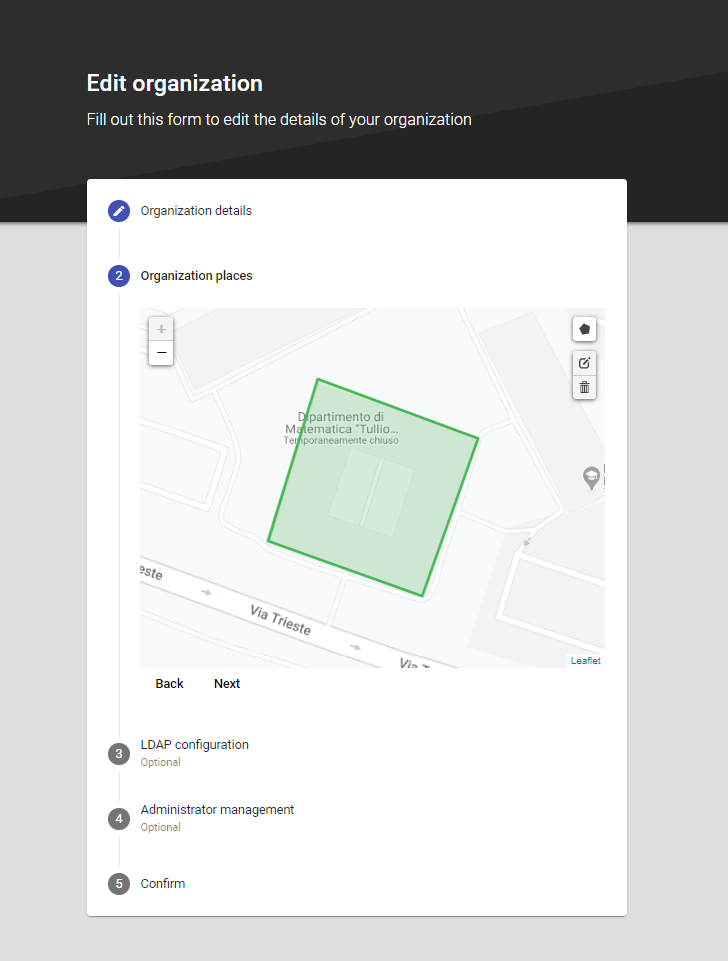
\includegraphics[width=120mm]{2-luoghi-organizzazione.png}
        \caption{Modifica luoghi dell'organizzazione}%
        \label{fig:web_app_modifica_luoghi_organizzazione}
    \end{figure}

    I luoghi si possono aggiungere, modificare ed eliminare direttamente dalla mappa interattiva, che si può ingrandire (+) oppure rimpicciolire (-) tramite i pulsanti in alto alla sinistra nella mappa.

    Per compiere azioni sulla mappa, ci sono tre pulsanti in alto a destra:
    \begin{itemize}
        \item cliccando il pulsante indicato con il poligono nero, si può creare un luogo bidimensionale sulla mappa cliccando con il tasto sinistro sui punti d'interesse. Per chiudere il poligono basta cliccare sul lato più adiacente all'ultimo punto cliccato dall'utente. Una volta creato il luogo, i dati relativi al luogo creato vengono rilevati attraverso \glossarioLocale{reverse geocoding}.
        \item cliccando il pulsante indicato con un foglio e una matita, si può modificare un luogo selezionandolo sulla mappa e modificando i vertici del poligono.
        \item cliccando il pulsante indicato con il cestino, si può eliminare un luogo selezionandolo sulla mappa.
    \end{itemize}

    Cliccando \textbf{Back} si torna al passaggio 1, mentre cliccando \textbf{Next} si va al passaggio 3.

    \item \textbf{LDAP configuration}-\textit{opzionale}

    \begin{figure}[H]
        \centering
        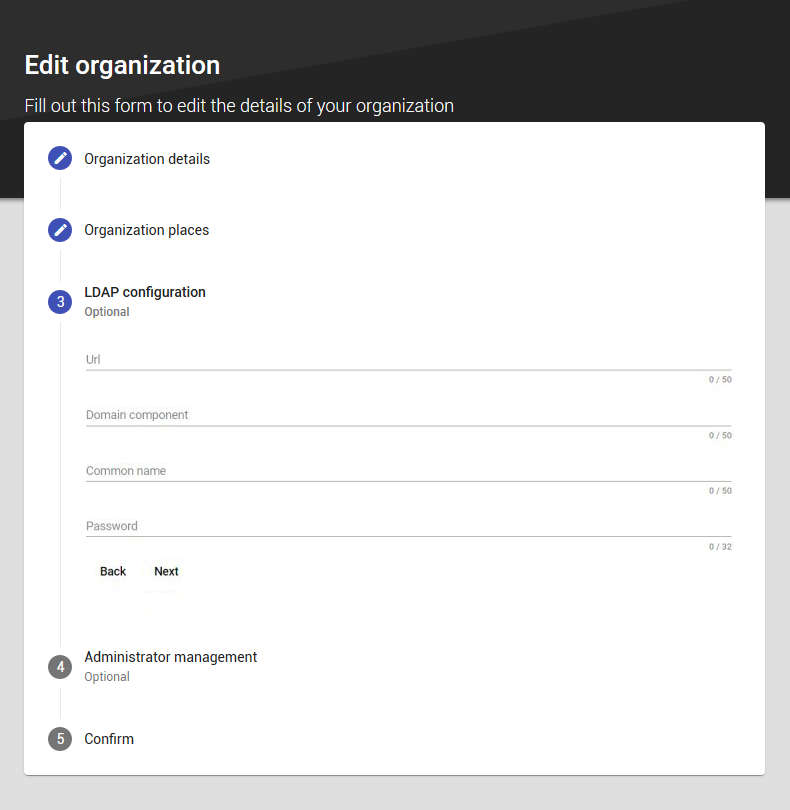
\includegraphics[width=120mm]{3-configurazione-ldap.png}
        \caption{Modifica configurazione LDAP}%
        \label{fig:web_app_modifica_configurazione_ldap}
    \end{figure}

    I campi che possono essere modificati sono:
    \begin{description}
        \item[Host] che corrisponde all'indirizzo IP del server LDAP per l'autenticazione.
        \item[Username] che è lo username per accedere all'organizzazione privata.
        \item[Password] che è la password per accedere all'organizzazione privata.
    \end{description}

    Cliccando \textbf{Back} si torna al passaggio 2, mentre cliccando \textbf{Next} si va al passaggio 4.

    \newpage
    \item \textbf{Administrator management}-\textit{opzionale}

    \begin{figure}[H]
        \centering
        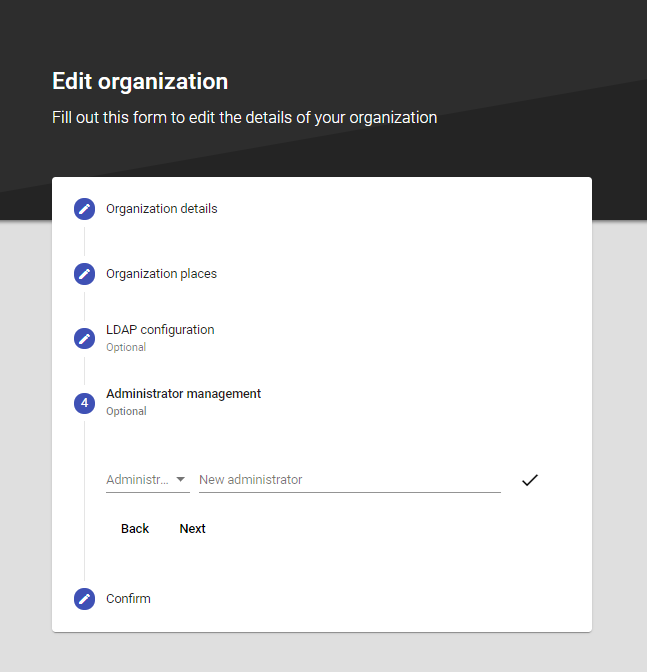
\includegraphics[width=120mm]{4-privilegi.png}
        \caption{Modifica privilegi utenti}%
        \label{fig:web_app_modifica_privilegi_utenti}
    \end{figure}

    Per aggiungere nuovi utenti con privilegi, si possono usufruire due campi di inserimento dati:
    \begin{itemize}
        \item un menu a tendina per la scelta della tipologia di utente, ovvero:
        \begin{itemize}
            \item \glossarioLocale{Administrator}.
            \item \glossarioLocale{Owner}.
            \item \glossarioLocale{Manager}.
            \item \glossarioLocale{Viewer}.
        \end{itemize}
        \item un campo dove aggiungere nome e cognome dell'utente del nuovo \glossarioLocale{amministratore}.
    \end{itemize}

    Una volta che questi dati sono stati inseriti correttamente, l'utente con i nuovi privilegi viene aggiunto cliccando sulla spunta che si trova a destra dei campi d'inserimento.
    % se l'utente inserito non esiste, che succede?? Aggiungere queste righe e che errori si possono verificare

    Non ci sono limiti per la ripetizione di questa procedura.

    Cliccando \textbf{Back} si torna al passaggio 3, mentre cliccando \textbf{Next} si va al passaggio 5.

    \newpage
    \item \textbf{Confirm}

    \begin{figure}[H]
        \centering
        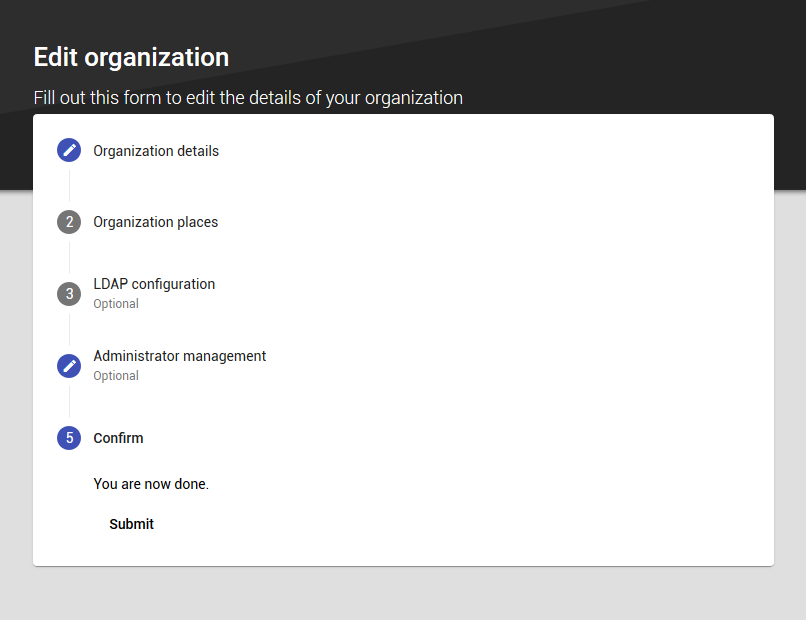
\includegraphics[width=120mm]{5-conferma-modifiche.png}
        \caption{Conferma modifiche}%
        \label{fig:web_app_conferma_modifiche}
    \end{figure}

    Questo è l'ultimo passaggio per la conferma delle modifiche effettuate. Per confermarle, basta cliccare la voce \textbf{Submit}.

\end{enumerate}
\newpage

% add other functionalities

\subsection{Risoluzione dei problemi}%
\label{subs:web_app_risoluzione_problemi}

\subsubsection{Accesso all'applicazione non disponibile}%
\label{subs:web_app_accesso_non_disponibile}

Nel caso ci siano problemi di collegamento alla web application, consigliamo di consultare il sito \textbf{http://www.isitdownrightnow.com/} per verificare se il problema riguarda il vostro provider oppure il nostro server.

Nel caso in problema sia legato al nostro server, vi preghiamo di riprovare l’accesso in un secondo momento.

Se il problema dovesse persistere, vi preghiamo di segnalarlo nelle modalità discusse nella sezione \textit{Supporto tecnico}.

\end{document}
